\documentclass[letterpaper, oneside, 11pt]{book}
\usepackage[left=1in, right=1in, top=0.75in]{geometry}
\usepackage[svgnames]{xcolor}
\usepackage{graphicx}
\usepackage{appendix}
\usepackage{float}
\usepackage{setspace}
\usepackage{acronym}
\usepackage[sfdefault]{roboto}
\usepackage{xcolor}
\usepackage{sectsty}
\usepackage[colorlinks=true, linkcolor=gray]{hyperref}
\usepackage[utf8]{inputenc}
\usepackage{hyperref}
\usepackage{tabularx}
\usepackage{longtable}
\usepackage{listings}
\usepackage{glossaries}

\setacronymstyle{long-short-desc}
\loadglsentries{defn}
\makenoidxglossaries

\definecolor{MyBlue}{rgb}{0.03, 0.27, 0.49}
\chapterfont{\color{MyBlue}}
\sectionfont{\color{MyBlue}}
\subsectionfont{\color{MyBlue}}
\setlength{\parindent}{0pt}

\begin{document}
%%========================================================================
\begin{titlepage}
	\raggedleft
	\begin{figure}[H]
	\centering
		\includegraphics[scale=1.53]{railway_track.jpg}
	\label{fig:track}
\end{figure}
	\vspace*{0.167\textheight}
	\textbf{\LARGE RSMS Installation and Operations Manual}\\[\baselineskip]
    \textbf{\textcolor{MyBlue}{\Huge R\Large ailway \Huge A\Large dministration and \Huge I\Large nformation \Huge L\Large ogical \Huge S\Large ystem}}\\[\baselineskip]
	{\Large \textit{RAILS for Model Railroads}}
	\vfill
    \vspace*{\baselineskip}
	{\small David Bristow}

	{\small Version 1.0.0}
	
	{\small January 20, 2025}
	\vspace*{3\baselineskip}
\end{titlepage}
%%========================================================================
\tableofcontents
%% copyright notice
%%========================================================================
\chapter{Microcontrollers for RAILS}
\section{Introduction}
\gls{rails} is a software model and implementation of an automated system to assist the model railroader achieve realism in the operation of a model railroad.
There are four user interface \gls{spa} that provide different aspects of rails they are:
\begin{itemize}
  \item \gls{rsrm} allows the user to match a rfid tag to a rollingstock's road name and number;
  \item \gls{mrim} allows the user to create, update and delete model railroad assets, such as rolling stock;
  \item \gls{mppm} allows the user to enter information about their projects and purchases; and
  \item \gls{mrlm} allows the user to enter information about their layout and control elements of it.
\end{itemize}
\section{RSRM Components}
The implementation of \gls{rsrm} consists of the following micro-services components:
\begin{itemize}
\item \gls{rfid} Controller is a micro-controller that processes \gls{rfid} tags obtained from a \gls{rfid} reader and then publishes \gls{iot} messages to the \gls{mqtt} Broker;
\item \gls{mqtt} Broker is responsible for receiving \gls{rfid} and micro info messages, filtering them, posting to designated topics and sending messages to clients subscribing to topics. The subscribers and publishers bridge the \gls{mqtt} elements with the GUI applications. The broker handles \gls{iot} messages;
\item \gls{isrs} subscribes to \gls{rfid} messages and pushes them via a web-socket to the rsm component;
\item \gls{isms} that subscribes to micro controller startup and heartbeat messages, updating the micros collection via \gls{rlds};
\item \gls{rlds} provides \gls{rest} access to model railroad layout collections including micros;
\item \gls{rids} provides \gls{rest} access to railroad inventory collections including rollingstock;
\item MongoDB a NoSQL database program that stores data records as documents which are gathered in collections. A database stores one or more collections of documents;
\item \gls{mr} Data is the document repository, used by MongoDB, to store complete collections of items such as rollingstock, industries (producers and consumers), track elements, turnouts, projects, purchases, etc. in support of \gls{rails}; and
\item \gls{rsrm} is the \gls{spa} that allows a user to match a \gls{rfid} tag to a rollingstock's road name and number.
\end{itemize}
Figure \ref{fig:rsms-ms-components} depicts the micro-services used to create the rolling stock \gls{rfid} management subsystem.

\begin{figure}[H]
	\centering
		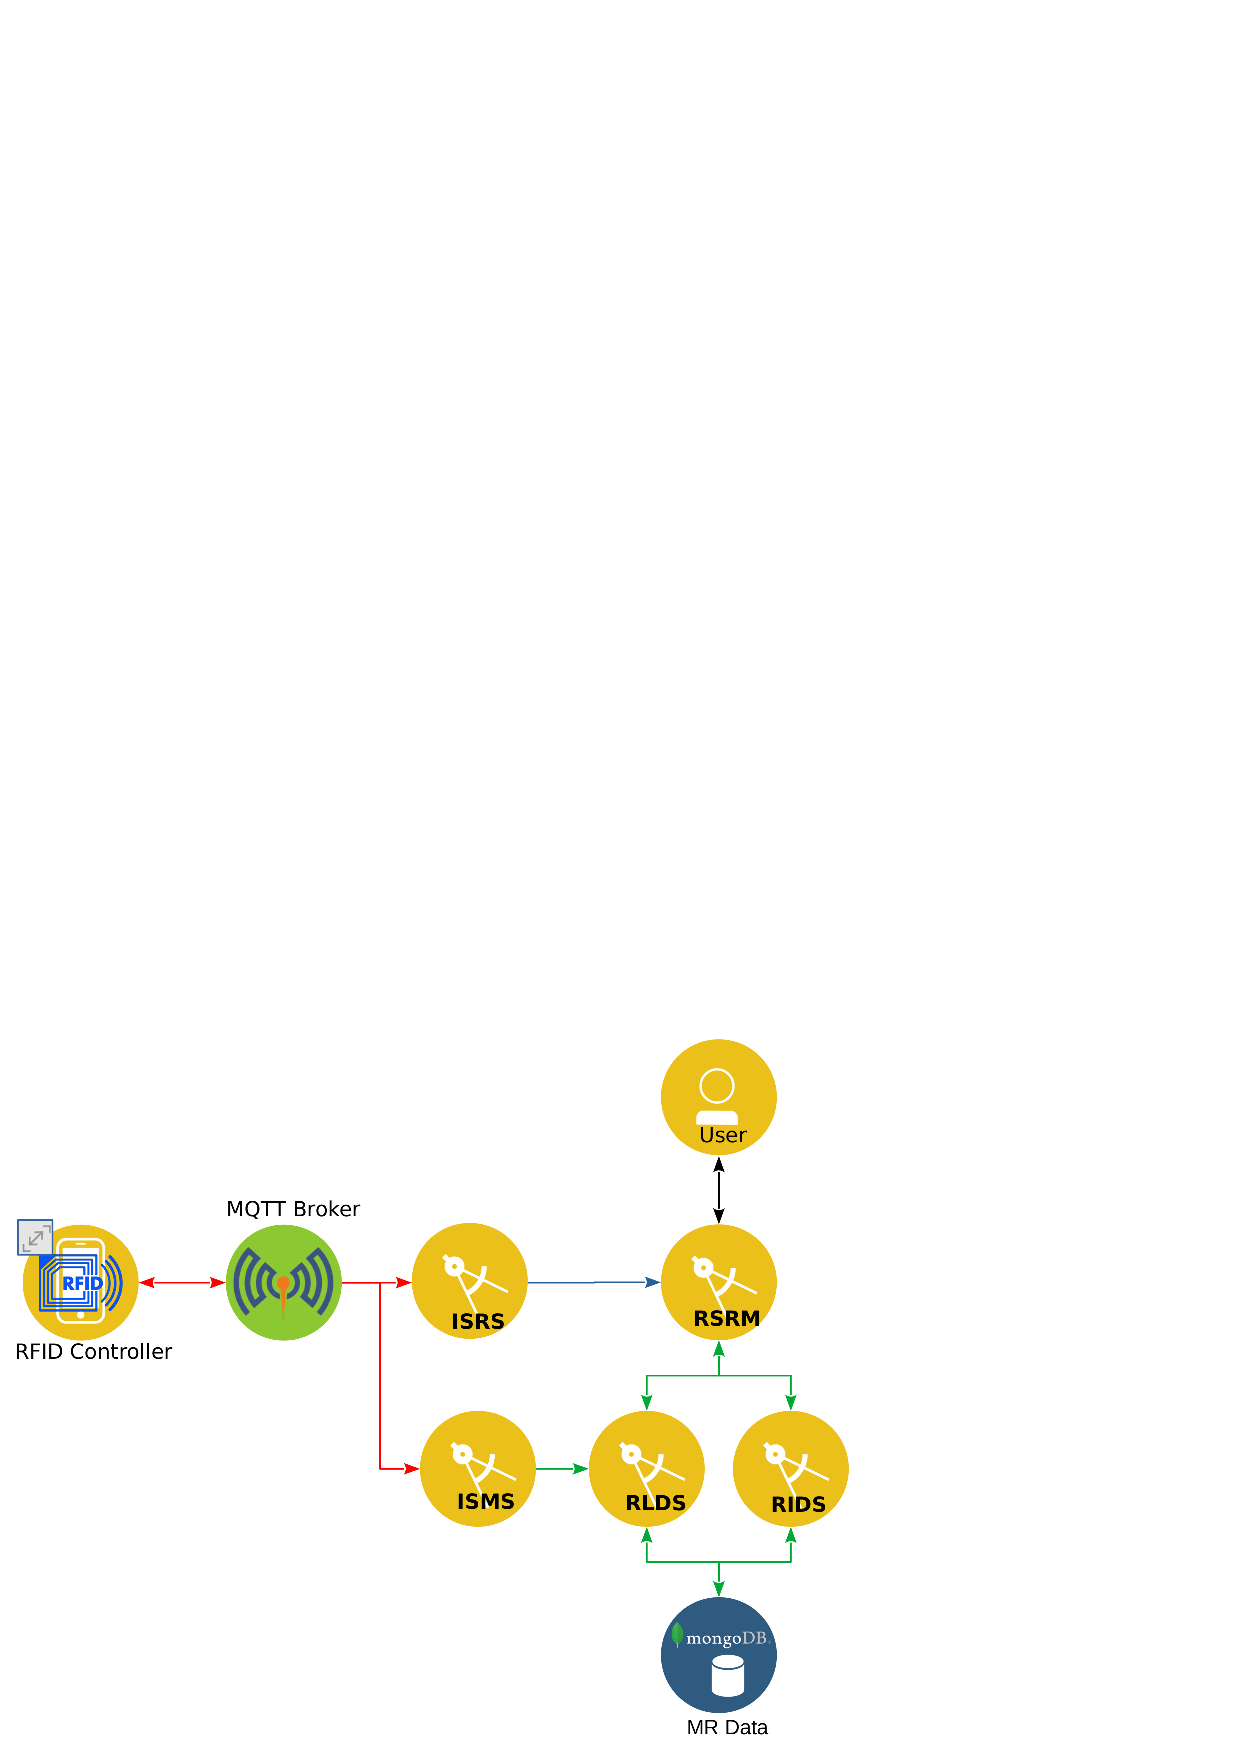
\includegraphics[scale=0.15]{rsms_design.png}
	\caption{Microservices Components}
	\label{fig:rsms-ms-components}
\end{figure}

Three system components that make up this subsystem:
\begin{itemize}
\item \gls{rfid} Controller is a micro-controller that processes \gls{rfid} tags obtained from a \gls{rfid} reader and then publishes \gls{iot} messages to the \gls{mqtt} Broker;
\item Network is a \gls{tcpip} communication medium that connects the \gls{rfid} Controller, \gls{mqtt} Broker and \gls{rsrm} components; and
\item Host is a computer that runs the \gls{mqtt} Broker and other \gls{rsrm} micro-services components.
\end{itemize}
Figure \ref{fig:rsms-system} depicts the systems components used to create the rolling stock \gls{rfid} management subsystem.

\begin{figure}[H]
	\centering
		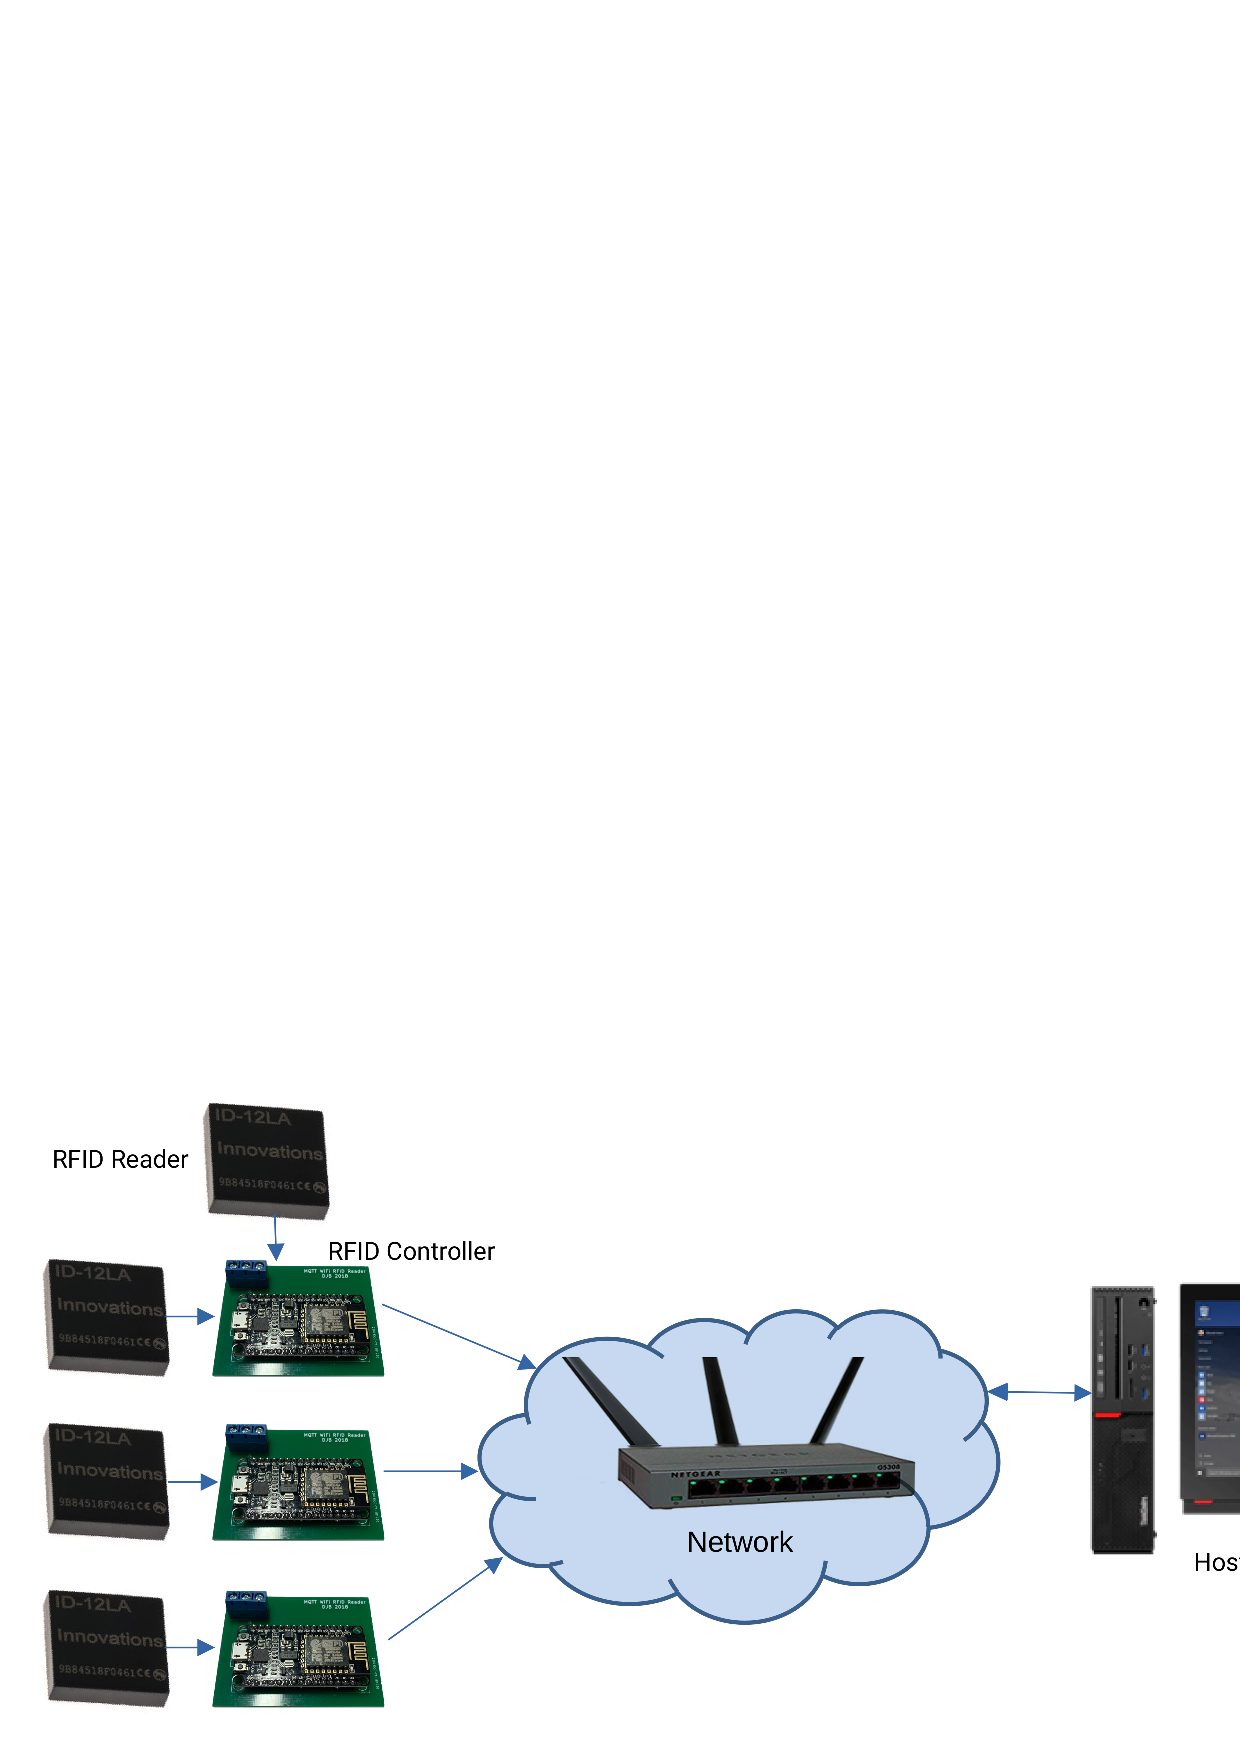
\includegraphics[scale=0.15]{rsms_system.png}
	\caption{MSystem Components}
	\label{fig:rsms-system}
\end{figure}

\section{MRLM System Components}

Figure \ref{fig:mrlm-ms-components} depicts the micro-services used to create the

\begin{figure}[H]
	\centering
		\includegraphics[scale=0.8]{mrlm_design.png}
	\caption{Microservices Components}
	\label{fig:mrlm-ms-components}
\end{figure}


\begin{figure}[H]
	\centering
		\includegraphics[scale=0.2]{turnout_system.png}
	\caption{MSystem Components}
	\label{fig:turnout-system}
\end{figure}
\chapter{RFID Reader Setup}

\section{Introduction}
Setting up an \gls{rfid} reader involves configuring both the hardware and software components to ensure proper communication and functionality. This guide will walk you through the necessary steps to 
set up your \gls{rfid} reader, including prerequisites, downloading the project from GitHub, modifying configuration files, building and uploading the code, and monitoring the serial output. 
By following these instructions, you will be able to integrate the RFID reader with your ESP8266-based development board and start using it for your applications.\\
\\
It is recommended to have a basic understanding of microcontrollers and familiarity with \gls{vscode} before proceeding with the setup. This knowledge will help you navigate the 
development environment and troubleshoot any potential issues that may arise.

\section{Prerequisites}
\begin{itemize}
    \item \gls{vscode}: Make sure you have \gls{vscode} installed on your system.
    \item PlatformIO IDE: Install the PlatformIO IDE extension for \gls{vscode}. This extension provides a powerful environment for developing and deploying code to various 
    microcontroller platforms, including ESP8266.
    \item Libraries: Ensure you have the necessary libraries installed. You can install them using PlatformIO. The required libraries are:
        \begin{itemize}
            \item `ESP8266WiFi`: Provides support for connecting to Wi-Fi networks.
            \item `PubSubClient`: Allows the ESP8266 to communicate with an \gls{mqtt} broker.
            \item `NTPClient`: Enables the ESP8266 to synchronize its clock with an \gls{ntp} server.
            \item `ArduinoJson`: Provides support for parsing and generating \gls{json} data.
        \end{itemize}
    \item ESP8266 Board: You'll need an ESP8266-based development board (e.g., NodeMCU, Wemos D1 Mini) connected to one or two \gls{rfid} readers.
    \item USB Cable: A micro-USB cable to connect your ESP8266 board to your computer.
\end{itemize}


\section{Downloading the Project from GitHub}
\begin{enumerate}
    \item Open \gls{vscode}
    \item Open the Command Palette: Press `Ctrl+Shift+P` (Windows/Linux) or `Cmd+Shift+P` (macOS).
    \item Type "Git: Clone" and select the option.
    \item Paste the GitHub repository URL\\ (https://github.com/djbristow/RAILS/tree/master/Microcontrollers/RFID/WiFi-RFID) into the input field.
    \item Choose a local directory to clone the project into.
\end{enumerate}

\section{Modifying the `params.h` File}
The `params.h` file contains configuration parameters that need to be set based on your specific setup. These parameters include the MQTT server address, port number, RFID reader identifier, 
Wi-Fi network credentials, and the number of RFID readers connected to the ESP8266 board. Follow these steps to modify the `params.h` file:
\begin{enumerate}
    \item Open the project directory in \gls{vscode}.
    \item Locate the `params.h` file within the project structure.
    \item Open the file in \gls{vscode}.
    \item Modify the following parameters as needed:
    \begin{itemize}
        \item `MQTTSERVER`: replace the 192.168.4.39 with the IP address of the \gls{mqtt} broker, ie the host computer.
        \begin{verbatim}
            #define MQTTSERVER "192.168.4.39"
        \end{verbatim}
        \item `MQTTPORT`: only replace the 1883 with the port number of the \gls{mqtt} if it is different.
        \begin{verbatim}
            #define MQTTPORT 1883
        \end{verbatim}
        \item `MQTTID`: replace the RfidRdr01 with a unique identifier for the \gls{rfid} reader. This identifier will be used to distinguish between different readers. It is recommended to use a naming convention 
        that helps identify the reader's purpose i.e 'RfidRdr' followed by a two digit number.
        \begin{verbatim}
            #define MQTTID "RfidRdr01" 
        \end{verbatim}
        \item `NUMBERREADERS`: replace the 1 with the number of RFID readers connected to the ESP8266 board, either 1 or 2.
        \begin{verbatim}
            #define NUMBERREADERS 1
        \end{verbatim}
        \item SSID: insert the SSID of your Wi-Fi network between the double quotes.
        \begin{verbatim}
            #define SSID ""
        \end{verbatim}
        \item PASSWORD: insert the password of your Wi-Fi network between the double quotes.
        \begin{verbatim}
            #define PASSWORD ""
        \end{verbatim}
    \end{itemize}
\end{enumerate}
Figure \ref{fig:params} shows the `params.h` file with the parameters that need to be modified. Make sure to save the file after making the changes.
\begin{figure}[H]
    \centering
    \includegraphics[scale=0.33]{./images/vsc-rfidsw.png}
    \caption{params.h File}
    \label{fig:params}
\end{figure}

\section{Building and Uploading the Code}
Once you have modified the `params.h` file with the necessary configuration parameters, you can build and upload the code to your ESP8266 board using PlatformIO. 
Follow these steps to build and upload the code:
\begin{enumerate}
    \item Connect your ESP8266 board to your computer using the micro-USB cable.
    \item Open the PlatformIO Home panel in \gls{vscode}.
    \item Select your ESP8266 board from the list of available boards. If your board is not listed, you may need to install the corresponding platform package.
    \item Click the "Build" button in the PlatformIO Home panel. This will compile the code into a binary file.
    \item Click the "Upload" button to upload the compiled code to your ESP8266 board.
\end{enumerate}
Figure \ref{fig:build} shows the `main.cpp` file with the code that will be uploaded to the ESP8266 board. Make sure to save the file before building and uploading the code.
The build icon is shown with a yellow arrow and the upload icon is shown with a green arrow in the PlatformIO Home panel.
\begin{figure}[H]
    \centering
    \includegraphics[scale=0.33]{./images/vsc-build.png}
    \caption{main.cpp File}
    \label{fig:build}
\end{figure}

\section{Monitoring the Serial Output (Optional)}
You can monitor the serial output of the ESP8266 board to debug any issues and observe the program's behavior. Follow these steps to monitor the serial output:
\begin{enumerate}
    \item Check that there is a \gls{rfid} reader connected to the ESP8266.
    \item Open the PlatformIO Serial Monitor in \gls{vscode}.
    \item Set the baud rate to match the baud rate used in your code (usually 115200).
    \item Observe the serial output to monitor the program's behavior and debug any issues.
    \item pass a \gls{rfid} tag over the RFID reader to see the output.
\end{enumerate}

\section{Operationalize the RFID Reader}
Once you have successfully uploaded the code to your ESP8266 board and verified that the \gls{rfid} reader is working correctly, you can start using it for your applications.
The \gls{rfid} reader will publish gls{rfid} tag data to the \gls{mqtt} broker, allowing other devices to subscribe to this data and perform various actions based on the received information.
\begin{enumerate}
    \item Install a \gls{rfid} reader under a scetion of track on your model railroad.
    \item Connect the \gls{rfid} reader to the ESP8266 board that has the code uploaded.
    \item Connect the ESP8266 board to a power source.
\end{enumerate}


\chapter{Docker Set Up}

\section{Docker Installation}
\label{sec:dockerinstall}
The \gls{rails} \glspl{spa} are implemented as Docker containers. The Docker containers are built and pushed to Docker Hub. The Docker containers are then pulled from Docker Hub and run on the host machine. 
The host machine must have Docker installed. Docker is a platform for developing, shipping, and running applications in containers. Docker can be installed on Windows, macOS, and Linux. 
The installation instructions for Docker can be found at \href{https://docs.docker.com/get-docker/}{https://docs.docker.com/get-docker/}.\\
\\
To see additioanl information on Docker installation of a complete \gls{rails} see \href{https://github.com/djbristow/RAILS/blob/master/Documentation/rails-docker.pdf}{Docker Implementation}.\\
\section{Broker Configuration}
\label{sec:brokerconfig}
The \gls{rails} \glspl{spa} use the Mosquitto broker to communicate with each other. The Mosquitto broker is an open-source message broker that implements the \gls{mqtt} protocol. The Mosquitto broker 
must be configured to allow the \gls{rails} \glspl{spa} to communicate with each other. The Mosquitto broker configuration file must be edited to allow the \gls{rails} \glspl{spa} to communicate with 
each other. The configuration file is found in the virtual storage whose volume name is “mosquitto”. To establish and modify the configuration file the following steps are taken:
\begin{enumerate}
    \item Create a Docker volume for the Mosquitto broker.
    \begin{verbatim}
    docker volume create --name mosquitto
    \end{verbatim}
    \item Run a Docker container for the first time the Mosquitto broker, which will create the initial configuration file.
    \begin{verbatim}
    docker run -it --name myMqttBrkr -p 1883:1883 -p 9001:9001 --rm
    -v mosquitto:/mosquitto -d eclipse-mosquitto
    \end{verbatim}
    \item Stop the broker container.
    \begin{verbatim}    
    docker stop myMqttBrkr
    \end{verbatim}
    \item Locate the configuration file in the "mosquitto" volume.
    \begin{verbatim}    
    docker inspect mosquitto
    \end{verbatim}
    \item Edit the configuration file modifying or adding the following lines:
    \begin{verbatim}
    listener 1883
    allow_anonymous true
    socket_domain ipv4
    \end{verbatim}
\end{enumerate}
\section{Create the RAILS Docker Environment}
\label{sec:railsdockerenv}
The \gls{rails} \glspl{spa} are implemented as Docker containers that require an environment to run in. To create that environment, the following steps are taken:
\begin{enumerate}
    \item Create a Docker volume for the Rails database.
    \begin{verbatim}
    docker volume create --name myRailsDb  
    \end{verbatim}
    \item Create a Docker volume for the Rails images.
    \begin{verbatim}
    docker volume create --name myRailsImages
    \end{verbatim}
    \item Create a Docker network for the Rails containers to communicate over.
    \begin{verbatim}
    docker network create myRailsNet
    \end{verbatim}
\end{enumerate}
\section{Run the RAILS Docker Containers}
\label{sec:railsdockercontainers}
The Docker containers are pulled from Docker Hub and run on the host machine. The following steps are taken to run the \gls{rails} Docker containers:
\begin{enumerate}
    \item Run a Docker container for the MongoDB database.
        \begin{verbatim}
        docker run --network myRailsNet --name myMongo -v myRailsDb:/data/db
        -p 27017:27017 -d mongo
        \end{verbatim}
    \item Run a Docker container for the \gls{rids} \gls{ds}.
        \begin{verbatim}
        docker run --network myRailsNet --name myRids -p 3000:3000 -d dbristow/rids
        \end{verbatim}
    \item Run a Docker container for the \gls{rlds} \gls{ds}.
        \begin{verbatim}
        docker run --network myRailsNet --name myRlds -p 3006:3006 -d dbristow/rlds
        \end{verbatim}
    \item Run a Docker container for the Mosquitto broker.
        \begin{verbatim}
        docker run --network myRailsNet -it --name myMqttBrkr -p 1883:1883 -p 9001:9001
        -v mosquitto:/mosquitto -d eclipse-mosquitto
        \end{verbatim}
    \item Run a Docker conatainer for the \gls{isrs} \gls{iots}.
        \begin{verbatim}
        docker run --network myRailsNet -p 3005:3005 --name myIsrs -d dbristow/isrs
        \end{verbatim}
    \item Run a Docker conatainer for the \gls{isms} \gls{iots}.
        \begin{verbatim}
        docker run --network myRailsNet --name myIsms -d dbristow/isms
        \end{verbatim}
    \item Run a Docker container for the \gls{rsrm} \gls{spa}.
        \begin{verbatim}
        docker run --network myRailsNet -p 3002:8080 --name myRsrm -d dbristow/rsrm
        \end{verbatim}
\end{enumerate}

To bring up the  \gls{rsrm} \gls{spa} point the browser to \href{http://localhost:3002}{http://localhost:3002}\\
\\
To stop the \gls{rails} Docker containers, the following command is used:
\begin{verbatim}  
    docker stop myRsrm myIsms myIsrs myRids myRlds myMongo myMqttBrkr
\end{verbatim}

To restart the \gls{rails} Docker containers, the following command is used:
\begin{verbatim}
    docker start myMongo myMqttBrkr myIsms myIsrs myRids myRsrm
\end{verbatim}

To remove the \gls{rails} Docker containers, the following commands are used:
\begin{verbatim}
    docker rm myRsrm myIsms myIsrs myRids myRlds myMongo myMqttBrkr
\end{verbatim}


\newcommand{\hamburger}{%
  \vbox{%
    \hrule width 1em height 1pt\smallskip
    \hrule width 1em height 1pt\smallskip
    \hrule width 1em height 1pt}%
}
\chapter{RSRM Operations}
\gls{rsrm} simplifies identifying rollingstock by associating \gls{rfid} tags with specific road names and numbers.
When a connected reader reads an \gls{rfid} tag, \gls{rsrm} searches its database for a matching entry. If a match is found, the application displays the corresponding 
road name and number of the rollingstock. If no match is found, the application provides input fields for the user to manually enter this information, 
creating a new association in the database.

\section{About Page}

The intial page when the application is opened in a web browser provides:
\begin{itemize}
    \item A version number of the application;
    \item A concise overview of the application's purpose and technology stack;
    \item The current database statistics indicating:
    \begin{itemize}
        \item The number of rollingstock entries in the database and how many have \gls{rfid} tags; and
        \item The number of micro-controllers in the database and how many are RFID readers.
    \end{itemize}
\end{itemize}
Figure \ref{fig:about1} shows the "About" page of the RAILS RS RFID Manager application.

\begin{figure}[H]
    \centering
    \includegraphics[scale=0.33]{./images/about.png}
    \caption{About Page}
    \label{fig:about1}
\end{figure}

The hamburger menu icon \hamburger, to the left of "RAILS" represents a hidden navigation menu that can be toggled open and closed. 
When the icon is clicked or tapped on the menu for navigation to different pages of this application is revealed. This menu  
contains the links: "Reader," "Admin," "Rollingstock," "AAR Codes," "About" (this page). 
Figure \ref{fig:about2} shows the "About" page with the navigation menu opened.

\begin{figure}[H]
    \centering
    \includegraphics[scale=0.33]{./images/about-sidemenu.png}
    \caption{Sidemenu}
    \label{fig:about2}
\end{figure}

\section{Reader Page}
This page displays a log of recently read \gls{rfid} tags and their associated information. It provides real-time or near real-time 
tracking of rolling stock as they pass over \gls{rfid} readers. To access the "RFID Tags Read" page from the main navigation menu on the 
left side of the screen, click on the "Reader" link. The "RFID Tags Read" page will be displayed.\\
\\
Figure \ref{fig:reader1} shows the initial "RFID Tags Read" page of the \gls{rsrm} application. Table displayed columns are:
\begin{itemize}
    \item Time: The date and time the \gls{rfid} tag was read;
    \item Sensor: The name of the micro-controller the \gls{rfid} reader is connected to;
    \item Reader: The identifier of the \gls{rfid} reader that detected the tag;
    \item Road Name and Number: This column has three possible entries:
    \begin{itemize} 
        \item "No data avaibale" indicates that no \gls{rfid} reader has sent any data to the \gls{rsrm} application;
        \item The road name and number of the rollingstock associated with the read \gls{rfid} tag.
        \item "Not registered" indicates that the \gls{rfid} tag was not found in the database.
    \end{itemize}
    \item AAR: The AAR code represents the type of rollingstock;
    \item Color: The color of the rollingstock;
    \item Register: If the \gls{rfid} tag is not in the database an icon appears that the user may click to add the associated 
    rollingstock to the database.
\end{itemize}
In the top left corner below the title is an \gls{rfid} icon that indicates the status of the \gls{rsrm} applications's connection to 
the \gls{mqtt} broker, green shows a good connection and red a failed connection.\\
The "CLEAR" button reloads the page and clears the log of read \gls{rfid} tags.
\begin{figure}[H]
    \centering
    \includegraphics[scale=0.33]{./images/reader.png}
    \caption{Initial RFID Tags Read Page}
    \label{fig:reader1}
\end{figure}
Figure \ref{fig:reader2} displays a log of with actual data read RFID tags and their associated information. The user can see that 
some tags are associated with known rollingstock ("CN 521491," "SCOX 1408," "CN 114520"), while others are marked as "Not Registered." 
This indicates that these tags are not yet linked to any rolling stock in the system's database. This is important for identifying 
new or unknown rollingstock. The user can click on the "Register" icon to add the rollingstock to the database.

\begin{figure}[H]
    \centering
    \includegraphics[scale=0.33]{./images/reader1.png}
    \caption{RFID Tags Read}
    \label{fig:reader2}
\end{figure}

When an RFID tag is read by a reader but is not found in the system's database, the "RFID Tags Read" section will display 
"Not Registered" in the "Road Name and Number" column. To associate this tag with a piece of rolling stock, the user may wish 
to register it. To do so, the user can click on the "Register" icon in the "Register" column. This action will open a dialog 
box where the user can enter the necessary information to create a new association between the RFID tag and the rolling stock. 
Once the information is saved, the new entry will be added to the database, and the "Not Registered" status will be updated to 
reflect the newly registered rolling stock.\\
\\
Figure \ref{fig:reader3} displays the "Rollingstock Registration" dialog box. It allows the user to associate the unregistered 
\gls{rfid} to a rollingstock to the system. The dialog box has:
\begin{itemize}
    \item Road Name: Enter the name of the railroad company or owner of the rollingstock;
    \item Road Number: Enter the unique identifying number assigned to the specific piece of rollingstock;
    \item two buttons:
    \begin{itemize}
        \item CANCEL: Closes the dialog box without saving the association to a rollingstock; and
        \item SAVE: Adds the \gls{rfid} tag to the identified rollingstock.
    \end{itemize}
\end{itemize}
\begin{figure}[H]
    \centering
    \includegraphics[scale=0.33]{./images/reader2.png}
    \caption{Revised RFID Tags Read}
    \label{fig:reader3}
\end{figure}
When the user clicks on the "SAVE" button, the dialog box will close, and adds the \gls{rfid} tag to the identified rollingstock 
and displayed in the "RFID Tags Read" page as shown in Figure \ref{fig:reader4}.
\begin{figure}[H]
    \centering
    \includegraphics[scale=0.33]{./images/reader3.png}
    \caption{Rollingstock Registration}
    \label{fig:reader4}
\end{figure}
If the user enters a road name and number that does not exist in the system's database, the system will expand the dialog box to allow 
the user to create a new rollingstock entry. The expanded dialog box, as shown in figure \ref{fig:reader6} has additional fields for the user to enter:
\begin{itemize}
    \item AAR: Select the AAR code corresponding to the rollingstock type from a dropdown list;
    \item Color: Enter the color of the rollingstock;
    \item along with the two buttons:
    \begin{itemize}
        \item CANCEL: Closes the dialog box without saving the new rollingstock; and
        \item SAVE: Saves the information entered and adds the new rollingstock to the database.
    \end{itemize}
\end{itemize}
\begin{figure}[H]
    \centering
    \includegraphics[scale=0.33]{./images/reader4.png}
    \caption{Expanded Rollingstock Registration}
    \label{fig:reader5}
\end{figure}
When the user clicks on the "SAVE" button, the dialog box will close, and adds the new rollingstock to the database
and displayed in the "RFID Tags Read" page as shown in Figure \ref{fig:reader6}.
\begin{figure}[H]
    \centering
    \includegraphics[scale=0.33]{./images/reader5.png}
    \caption{RFID Tags Read}
    \label{fig:reader6}
\end{figure}

\section{Admin Page}
This page allows the user to manage the RFID readers (micro-controllers) connected to the system. To access the "Admin RFID Micros" page 
from the main navigation menu on the left side of the screen, click on the "Admin" link. The "Admin RFID Micros" page will be displayed. 
While the focus of the \gls{rsrm} "Admin RFID Micros" page is on managing \gls{rfid} micro-controllers any micro-controller can be managed.
Figure \ref{fig:admin1} shows the "Admin RFID Micros" page of the \gls{rsrm} application. Table displayed columns are:
\begin{itemize}
    \item Name: The name of the micro-controller (e.g., RfidRdr00, ToCntlr01, RfidRdr03);
    \item IP Address: The IP address of the micro-controller;
    \item Date Time: The last recorded communication both data and heartbeat messages time with the micro-controller;
    \item Location: The physical location on the layout of the micro-controller sensor (\gls{rfid} reader);
    \item Status: An indicator of the reader's current status, represented by a color-coded icon:
    \begin{itemize}
        \item Green: Reader is active and communicating correctly.
        \item Yellow: Reader is connected but may have issues or hasn't communicated recently.
        \item Red: Reader is not communicating or is offline.
    \end{itemize}
    \item Actions: This column contains icons, for editing and deleting an existing micro-controller:
    \begin{itemize}
        \item Clicking the "Edit" (pencil) icon will open a dialog box allowing the user to modify the micro-controller's information; and
        \item Clicking the "Delete" (trash can) icon will remove the micro-controller entry from the system. A confirmation dialog box will 
        appear to prevent accidental deletions.
    \end{itemize}
\end{itemize}

Clicking on any of the table headers, except the "Actions" header, sorts the list by that header alphanumerically, either forward or reverse. For example 
if the user clicked on the "IP" header the entire list of micro-controllers would be sorted by their IP attribute. An arrow appears to the right of the 
header indicating which diretion the sort occurs.\\
\\
This table is paginated, showing the group of rollingstocks displayed (e.g. "1-5") and the total number of rollingstocks (e.g. "5") conatined in the database, along 
with navigation buttons ("<" and ">") to move between pages. The user can also select the number of items to display per page, where the default setting is 10.
The "ADD MICRO" button allows the user to add new rollingstock to the system.\\
\\
The "EXPORT RFID RS" Button exports the rollingstock data containing all of the rollingstock attributes to a CSV file.\\
\\
The "PRINT RFID REPORT" Button generates a printable \gls{pdf} report of the rollingstock data containing \gls{rfid}, Road Name, Road Number, Color, \gls{aar} Code, 
and Description of the rollingstock attributes.

\begin{figure}[H]
    \centering
    \includegraphics[scale=0.33]{./images/admin.png}
    \caption{Admin Page}
    \label{fig:admin1}
\end{figure}

Figure \ref{fig:admin2} shows a dialog box, which is accessed by clicking the "ADD MICRO" button in the "Admin RFID Micros" page. It allows the user to add 
a new entry for rollingstock to the system. The dialog box has:
\begin{itemize}
    \item Name: Enter the name of the micro-controller (e.g., RfidRdr00, ToCntlr01, RfidRdr03);
    \item IP Address: Enter the IP address of the micro-controller;
    \item Time: Enter a time in \gls{epoch} format;
    \item Purpose: Enter the purpose of the micro-controller (e.g., RFID Reader, Turnout Controller, RFID Reader);
    \item Location: Enter the physical location on the layout of the micro-controller sensor (e.g., \gls{rfid} reader);
    \item Status: Enter the micro-controller's current status (e.g., Up, Problem, Down).
\end{itemize}
The dialog box also has two buttons:
\begin{itemize}
    \item CANCEL: Closes the dialog box without saving the new micro-controller; and
    \item SAVE: Saves the information entered and adds the new micro-controller to the database and the new micro-controller will appear in the list.
\end{itemize}

\begin{figure}[H]
    \centering
    \includegraphics[scale=0.33]{./images/admin-micro-add.png}
    \caption{Admin Page}
    \label{fig:admin2}
\end{figure}

Figure \ref{fig:admin3} shows the "Micro" edit dialog box. It displays the details of an existing a micro-controller that 
the user clicked or tapped the pencil icon on. This dialog box has the same fields and buttons as the "New Micro" dialog box, 
but the SAVE button modifies the existing record in the database instead of creating a new one.

\begin{figure}[H]
    \centering
    \includegraphics[scale=0.33]{./images/admin-micro-edit.png}
    \caption{Admin Page}
    \label{fig:admin3}
\end{figure}

\section{Rollingstock Page}
This page provides a searchable and manageable list of all rollingstocks tracked by the system. To access the "Rollingstock" page 
from the main navigation menu on the left side of the screen, click on the "Rollingstock" link. The "Inventory of Rollingstock" view will be displayed.
Figure \ref{fig:rollingstock1} shows the "Rollingstock" page of the \gls{rsrm} application. Table displayed columns are:
\begin{itemize}
    \item Road Name: The name of the railroad company or owner of the rollingstock (e.g., ACFX, ADCX, ALNX, ALPX).
    \item Road Number: The unique identifying number assigned to the specific piece of rollingstock (e.g., 44763, 5425, 396029).
    \item \gls{aar}: The AAR code represents the type of rollingstock (e.g., LO, RM).
    \item Color: The color of the rollingstock (e.g., Grey, White, Blue).
    \item \gls{rfid}: The unique identifier of the \gls{rfid} tag associated with the rollingstock.
    \item Actions: This column contains icons, for editing and deleting an existing AAR code:
    \begin{itemize}
        \item Clicking the "Edit" (pencil) icon will open a dialog box allowing the user to modify the rollingstock's information; and
        \item Clicking the "Delete" (trash can) icon will remove the rollingstock entry from the system. A confirmation dialog box will 
        appear to prevent accidental deletions.
    \end{itemize}
\end{itemize}

A search bar (labeled with a magnifying glass icon and "Search") allows the user to filter the list of rollingstock by various strings (regradless of case). 
The table will automatically filter to display only entries that match your search. The search is performed across all displayed columns (Road Name, Road 
Number, AAR, Color, RFID). The following are some search examples:
\begin{itemize}
    \item Searching for "ACFX" or "acfx" will display all rollingstock with the Road Name "ACFX";
    \item Searching for "44" will display the rollingstock containing the Road Number "44" including "44763";
    \item Searching for "Blue" will display all blue rollingstock.
\end{itemize}
    
Clicking on any of the table headers, except the "Actions" header, sorts the list by that header alphanumerically, either forward or reverse. For example if 
the user clicked on the "Color" header the entire list of rollingstocks would be sorted by their color attribute. An arrow appears to the right of the 
header indicating which diretion the sort occurs.\\
\\
This table is paginated, showing the group of rollingstocks displayed (e.g. "1-10") and the total number of rollingstocks (e.g. "211") contained in the database, along 
with navigation buttons ("<" and ">") to move between pages. The user can also select the number of items to display per page, where the default setting is 10.
The "NEW ROLLINGSTOCK" button allows the user to add new rollingstock to the system.

\begin{figure}[H]
    \centering
    \includegraphics[scale=0.33]{./images/rs.png}
    \caption{Rollingstock Page}
    \label{fig:rollingstock1}
\end{figure}

Figure \ref{fig:rollingstock2} shows a dialog box, which is accessed by clicking the "NEW ROLLINGSTOCK" button in the "Inventory of Rollingstock" page. It allows the user to add 
a new entry for rollingstock to the system. The dialog box has:
\begin{itemize}
    \item twenty four input fields;
    \begin{itemize}
        \item Road Name (required): Enter the name of the railroad company or owner of the rollingstock;
        \item Road Number (required): Enter the unique identifying number assigned to the specific piece of rollingstock;
        \item AAR (required): Enter the AAR code corresponding to the rollingstock type;
        \item Color: Enter the color of the rollingstock (e.g., "Grey," "Blue," "Red");
        \item Description: Enter any additional descriptive information about the rollingstock;
        \item Number Built: Enter the total number of units built in this series;
        \item Builder: Enter the name of the manufacturer who built the rollingstock;
        \item Built Date: Enter the date the rollingstock was built;
        \item In Service Date: Enter the date the rollingstock was put into service;
        \item Inside Length, Inside Height, Inside Width, Lt Weight: Enter these fields as they are are specific to certain types of rollingstock. They are used to record relevant dimensions and weight information.
        \item Load Limit: Enter the maximum weight capacity of the rollingstock;
        \item Load Types: Enter the types of cargo the rollingstock is designed to carry (e.g., "General Merchandise," "Coal," "Automobiles");
        \item Capacity: Enter the rollingstock's specific capacity (e.g., "100 tons," "50 cars," etc.);
        \item Home Location: Enter where the rollingstock is typically based or maintained;
        \item Last Maintenance: Enter the date of the last maintenance performed on the rollingstock;
        \item Status: Enter the rollingstock's current operational status (e.g., "In Service," "Out of Service," or "Maintenance”);
        \item RFID Tag: Enter the unique identifier of the RFID tag associated with the rollingstock;
        \item Weight: Enter the weight of the model rollingstock;
        \item Length: Enter the length of the model rollingstock;
        \item Image ID: Enter an identifier for an associated image of the rollingstock; and
        \item Notes: Enter any additional notes or observations about the rollingstock.
    \end{itemize}
    \item two buttons:
    \begin{itemize}
        \item CANCEL: Closes the dialog box without saving the new rollingstock; and
        \item SAVE: Saves the information entered and adds the new rollingstock to the database and the new code will appear in the rollingstock list.
    \end{itemize}
\end{itemize} 
\begin{figure}[H]
    \centering
    \includegraphics[scale=0.33]{./images/rs-add.png}
    \caption{Rolling Stock Page}
    \label{fig:rollingstock2}
\end{figure}

Figure \ref{fig:rollingstock3} shows the "Rollingstock" edit dialog box. It displays the details of an existing a rollingstock that 
the user clicked or tapped the pencil icon on. This dialog box has the same fields and buttons as the "New Rolling Stock" dialog box, 
but the SAVE button modifies the existing record in the database instead of creating a new one.

\begin{figure}[H]
    \centering
    \includegraphics[scale=0.33]{./images/rs-edit.png}
    \caption{Rolling Stock Page}
    \label{fig:rollingstock3}
\end{figure}

\section{AAR Code Page}
This page provides a manageable list of \gls{aar} car codes, standardized codes used to classify different types of railroad cars, allowing users to understand 
the different types of railroad cars the system tracks. To access the "AAR Code" page from the main navigation menu on the left side of the screen, click on 
the "AAR Codes" link. Then "AAR Codes" page will be displayed.\vspace{5mm} \\
\\
Figure \ref{fig:aar1} shows the "AAR Codes" page of the \gls{rsrm} application. Table displayed columns are:
\begin{itemize}
    \item \gls{aar}: The \gls{aar} code (e.g., BE, BMR, DA).
    \item \gls{rs} Type: The general type of rollingstock (e.g., Passenger, Freight, Locomotive).
    \item Description: A detailed description of the car type.
    \item Actions: This column contains icons, for editing and deleting an existing AAR code:
    \begin{itemize}
        \item Clicking the "Edit" (pencil) icon will open a dialog box allowing the user to modify the \gls{aar} Code's information; and
        \item Clicking the "Delete" (trash can) icon will remove the \gls{aar} code entry from the system. A confirmation dialog box will 
        appear to prevent accidental deletions.
    \end{itemize}
\end{itemize}

Clicking on any of the table headers, except the "Actions" header, sorts the list by that header alphanumerically, either forward or reverse. For example 
if the user clicked on the "RS Type" header the entire list of \gls{aar} codes would be sorted by their \gls{rs} type attribute. An arrow appears 
to the right of the header indicating which diretion the sort occurs. \\
\\
This table is paginated, showing the group of AAR Codes displayed (e.g. "1-10") and the total number of AAR Codes (e.g. "34") conatined in the database, along 
with navigation buttons ("<" and ">") to move between pages. The user can also select the number of items to display per page, where the default setting is 10.
The "ADD AAR CODE" button allows the user to add new \gls{aar} codes to the system.
   
\begin{figure}[H]
    \centering
    \includegraphics[scale=0.33]{./images/aar.png}
    \caption{AAR Code Page}
    \label{fig:aar1}
\end{figure}

Figure \ref{fig:aar2} shows a dialog box, which is accessed by clicking the "ADD AAR CODE" button in the "AAR Codes" page. It allows the user to add 
a new entry for \gls{aar} Code to the system. 
The dialog box has:
\begin{itemize}
    \item three input fields, \gls{aar} Code, RS Type, and Description;
    \item two buttons:
    \begin{itemize}
        \item CANCEL: Closes the dialog box without saving the new \gls{aar} code; and
        \item SAVE: Saves the information entered and adds the new \gls{aar} code to the database and the new code will appear in the \gls{aar} Codes list.
    \end{itemize}
\end{itemize} 

\begin{figure}[H]
    \centering
    \includegraphics[scale=0.33]{./images/aar-add.png}
    \caption{Add AAR Code Dialog Box}
    \label{fig:aar2}
\end{figure}

Figure \ref{fig:aar3} shows the "AAR Code" edit dialog box. It displays the details of an existing \gls{aar} code that 
the user clicked or tapped the pencil icon on. This dialog box has the same fields and buttons as the "New AAR Code" dialog box, 
but the SAVE button modifies the existing record in the database instead of creating a new one.

\begin{figure}[H]
    \centering
    \includegraphics[scale=0.33]{./images/aar-edit.png}
    \caption{Edit AAR Code Dialog Box}
    \label{fig:aar3}
\end{figure}

%%========================================================================
\backmatter

\printnoidxglossary[sort=letter]
\addcontentsline{toc}{chapter}{Glossary}

\end{document}
